\chapter{狭义相对论}
\section{4维表述基础}
\subsection{预备知识}
不论是否发生了什么,空间的一点和时间的一瞬的结合就叫一个\textcolor{blue}{事件}(event).全部事件的集合叫\textcolor{blue}{时空}(spacetime).狭义相对论中谈及的\textcolor{blue}{粒子}(particle)是模型化语言,是完全没有大小的点,分为有静质量的粒子(质点)和无静质量的粒子(光子,photon)两类.一个粒子的全部历史由一系列事件组成,因此对应于时空中的一条曲线,称为该粒子的\textcolor{blue}{世界线}(world line),如图\ref{fig:6-1}所示.
\begin{figure}[htbp]
    \centering
 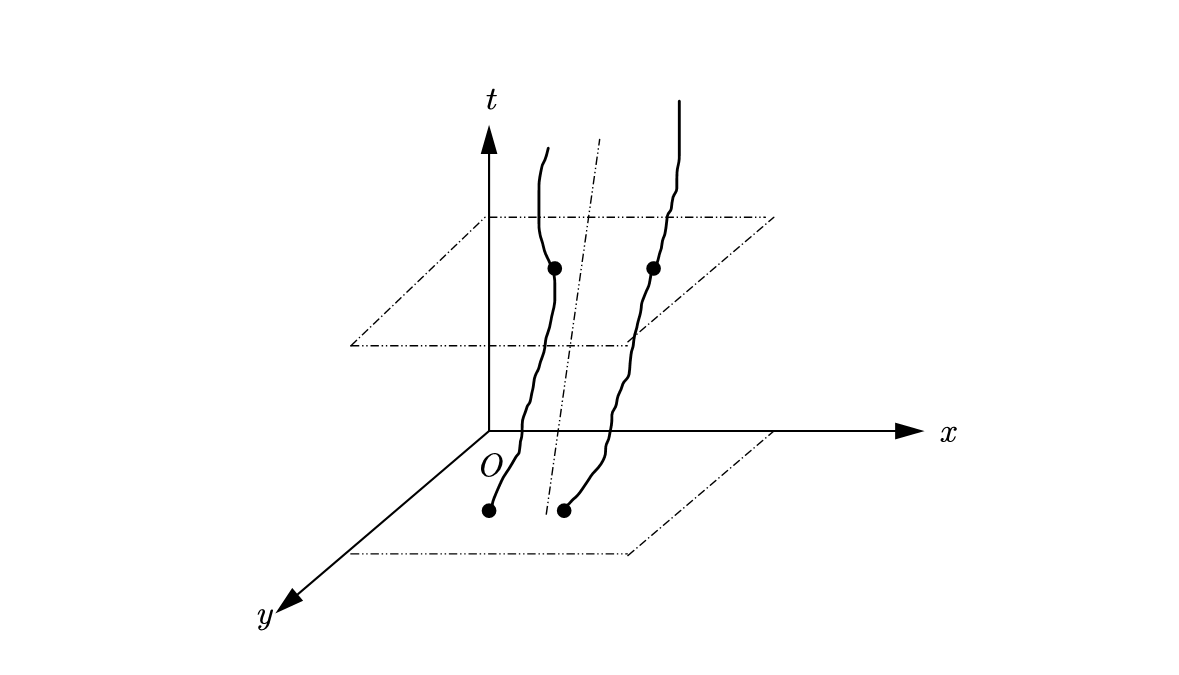
\includegraphics[width=0.8\textwidth]{img/6-1.png}
    \caption{世界线}
    \label{fig:6-1}
\end{figure}

进行物理观测的人叫观察者,将之模型化看成质点,简称\textcolor{blue}{观者}.为了观测,观者手中应有一个走时准确的钟,叫\textcolor{blue}{标准钟}(standard clock),该钟的读数称为该观者的\textcolor{blue}{固有时}(proper time).固有时$\tau$无非是质点世界线的一个特殊参数.
无数观者的集合$\mathscr{R}$叫一个\textcolor{blue}{参考系}(reference frame),满足时空或其一个开子集中的任一点有且仅有$\mathscr{R}$内的一个观者的世界线经过.参考系即世界线的线汇,即对于参考系
\begin{itemize}
\item 过任意事件均有一条世界线.
\item 世界线不相交.
\end{itemize}

\begin{figure}[htbp]
    \centering
 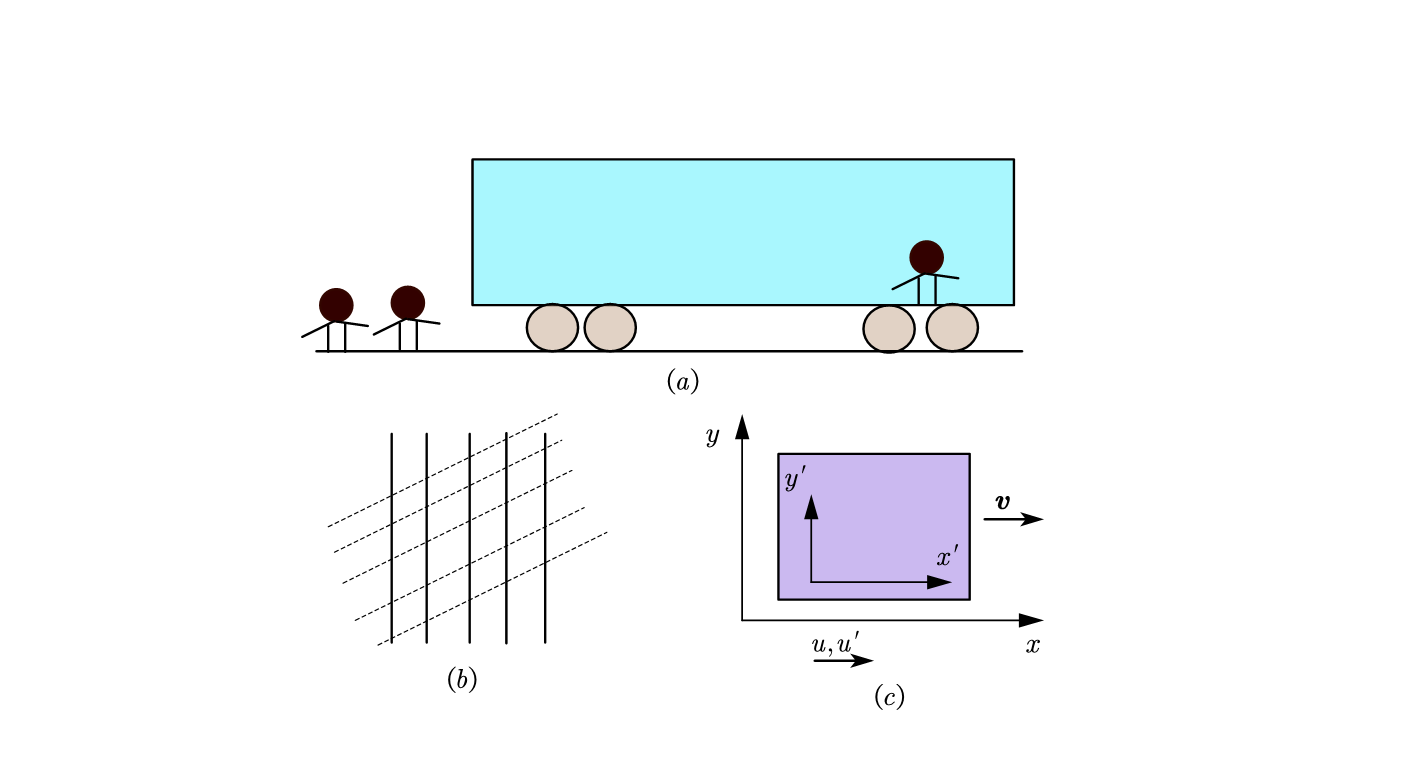
\includegraphics[width=1.2\textwidth]{img/6-2.png}
    \caption{(a):地面系和火车系示意图;(b):地面系(实线)和火车系(虚线)的世界线;(c):Galileo变换}
    \label{fig:6-2}
\end{figure}

如上图\ref{fig:6-2}所示,(a)代表火车系和地面系,而(b)中以许多竖直实线代表地面系观者们的世界线,火车系观者们的世界线则是许多互相平行的斜直虚线.(c)表示Galileo变换,与Galileo相对性原理(任两个惯性系都是平权的)构成Galileo的两大理论贡献.如(c)所示,Galileo变换的坐标变换公式为:
\begin{align}
    \left\{
    \begin{aligned}
        x^\prime&=x-vt\\
        y^\prime&=y\\
        z^\prime&=z\\
        t^\prime&=t
    \end{aligned}
    \right.
\end{align}
坐标变换公式中最后一式蕴含了同时性的绝对性.速度合成公式为:
\begin{align}
    \boldsymbol{u}^\prime=\boldsymbol{u}-\boldsymbol{v}.
\end{align}
\subsection{Maxwell方程的参考系问题}
Maxwell方程组表明Galileo相对性原理对于电磁理论并不成立.于是存在以下两种非此即彼的选择:
\begin{itemize}
\item 认为相对性原理并不总是成立的,即惯性系不平权.存在一个特殊的惯性系(以太,ether),其中光速为c,而其他惯性系则不然.
\item 坚持相对性原理总是成立的.
\end{itemize}

\begin{figure}[htbp]
    \centering
 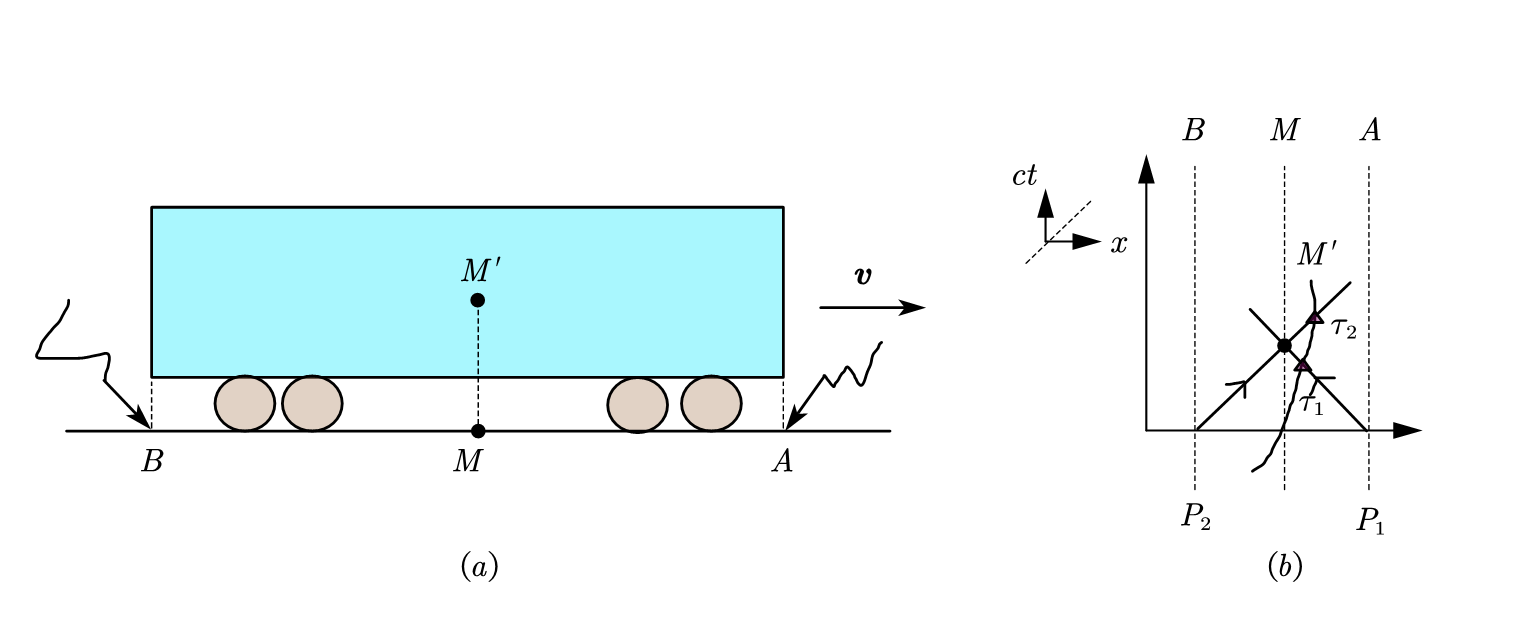
\includegraphics[width=\textwidth]{img/6-3.png}
    \caption{(a):闪电击中车头和车尾;(b):利用世界线进行分析}
    \label{fig:6-3}
\end{figure}

如图\ref{fig:6-3}(a),闪电分别击中火车车头$A$和车尾$B$,地面系$M$认为$A$和$B$同时遭受雷击,而火车系$M^\prime$认为并不同时,车头$A$首先遭受雷击.这表明了“同时的相对性”.以四维语言的时空图分析,地面系$M$的世界线为$P_2P_1$的中垂线,从$P_2,P_1$处发的光自然同时到达$M$.而火车系$M^\prime$的世界线却首先和$P_1$发出的光相遇(时间记为$\tau_1$),其次再和$P_2$相遇(时间记为$\tau_2$),所以$\tau_1<\tau_2$.

狭义相对论的两条假设为:
\begin{itemize}
\item 相对性原理
\item 光速不变性
\end{itemize}
并假设空间是均匀的,各向同性的.洛伦兹变换($v<c$,$c$取为1)为:
\begin{align}
    \left.
\begin{aligned}
    x^\prime&=\gamma(x-vt),\gamma=\dfrac{1}{\sqrt{1-v^2}}\\
    t^\prime&=\gamma(t-vx)
\end{aligned}
\right\}\Rightarrow
\left\{
\begin{aligned}
    u_x^\prime&=\dfrac{u_x-v}{1-u_xv}\\
    u_y^\prime&=\dfrac{u_y}{\gamma(1-u_xv)}\\
    u_z^\prime&=\dfrac{u_z}{\gamma(1-u_xv)}
\end{aligned}
\right.
\end{align}
另一个效果是间隔不变性:
\begin{align}
    \begin{aligned}
        \text{d}I^2&\equiv-\text{d}t^2+\text{d}x^2+\text{d}y^2+\text{d}z^2\\
        \text{d}I^{\prime2}&\equiv-\text{d}t^{\prime2}+\text{d}x^{\prime2}+\text{d}y^{\prime2}+\text{d}z^{\prime2}\\
        \text{d}I^2&=\text{d}I^{\prime2}
    \end{aligned}
\end{align}

\subsection{几何语言重新表述SR}
$$
\begin{aligned}
    \text{牛顿引力论}&\to (\mathbb{R}^4,?)\\
    \text{SR}&\to (\mathbb{R}^4,\eta_{ab})\\
    \text{GR}&\to (\underset{\underset{\text{联通的}}{\downarrow}}{M},g_{ab})
\end{aligned}
\Rightarrow
\left\{
\begin{aligned}
\overset{\underset{}{\text{物理}}}{\text{惯性系坐标}}&\to \overset{\underset{}{\text{数学}}}{\text{洛伦兹坐标}}\\
\text{间隔不变}&\to \text{线元不变}\\
\text{背景}&\to \text{闵氏时空}\\
\end{aligned}
\right.
$$
$$
\begin{aligned}
\overset{\boldsymbol{Phys.}}{inertial \ corrdinates} &\longleftrightarrow \overset{\boldsymbol{Math.}}{Lorentizian \ coordinates}\\
\underset{\text{间隔}}{interval}&\longleftrightarrow Minkowski\ line\ element\\
background\ spacetime &\longleftrightarrow 4-dim\ Minkowski \ space\\
observer(point mass) &\longleftrightarrow timelike\ curve\\
\underset{\text{惯性观者}}{inertial\quad observer}&\longleftrightarrow timelike\ geodesic
\end{aligned}
$$


